\documentclass[a4paper]{article}
\usepackage{amsmath}
\usepackage{fancyhdr}
\usepackage{graphicx}
\pagestyle{fancy}
\lfoot{Andrew Martin}
\rfoot{10/8/2017}
\begin{document}
	\title{Numerical Methods Assignment 1}
	\date{August 14, 2017}
	\author{Andrew Martin}
	\maketitle
	
		
	Question 1\\
	
	Given 3 potentially unevenly spaced points $$(x_j,f_j) ,(x_{j+1},f_{j+1}) , (x_{j+2},f_{j+2})$$ 
	
	The general Lagrange polynomial has form:
	$$p_n(x) = \sum_{j=0}^{n}f_jL_j(x),\qquad L_j(x)=\prod_{\substack{i=0\\i\neq j}}^{n}\frac{x-x_i}{x_j-x_i}$$
	
	So for quadratic polynomial interpolation we get:

	$$p_2(x) = f_j(\frac{x-x_{j+1}}{x_j-x_{j+1}})(\frac{x-x_{j+2}}{x_j-x_{j+2}})+
	f_{j+1}(\frac{x-x_{j}}{x_{j+1}-x_{j}})(\frac{x-x_{j+2}}{x_{j+1}-x_{j+2}})
	+ 
	f_{j+2} (\frac{x-x_{j}}{x_{j+2}-x_{j}})(\frac{x-x_{j+1}}{x_{j+2}-x_{j+1}})$$
	
	So the first derivative of this will be given by:
	$$p_2'(x)=\frac{d}{dx}\left[f_j(\frac{x-x_{j+1}}{x_j-x_{j+1}})(\frac{x-x_{j+2}}{x_j-x_{j+2}})+
	f_{j+1}(\frac{x-x_{j}}{x_{j+1}-x_{j}})(\frac{x-x_{j+2}}{x_{j+1}-x_{j+2}})
	+ 
	f_{j+2} (\frac{x-x_{j}}{x_{j+2}-x_{j}})(\frac{x-x_{j+1}}{x_{j+2}-x_{j+1}})\right]$$
	Noting that $f_n$, $x_k$ are constants
	
	$$\implies p_2'(x)=\frac{d}{dx}\left[f_j(\frac{x-x_{j+1}}{x_j-x_{j+1}})(\frac{x-x_{j+2}}{x_j-x_{j+2}})+
	f_{j+1}(\frac{x-x_{j}}{x_{j+1}-x_{j}})(\frac{x-x_{j+2}}{x_{j+1}-x_{j+2}})
	+ 
	f_{j+2} (\frac{x-x_{j}}{x_{j+2}-x_{j}})(\frac{x-x_{j+1}}{x_{j+2}-x_{j+1}})\right]$$
	
$$p_2'(x)=
\frac{f_j}{(x_j-x_{j+1})(x_j-x_{j+2})}\frac{d}{dx}\left[(x-x_{j+1})(x-x_{j+2})\right] +
\frac{f_{j+1}}{(x_{j+1}-x_{j})(x_{j+1}-x_{j+2})}\frac{d}{dx}\left[(x-x_{j})(x-x_{j+2})\right]+
\frac{f_{j+2}}{(x_{j+2}-x_{j})(x_{j+2}-x_{j+1})}\frac{d}{dx}\left[(x-x_{j})(x-x_{j+1})\right]$$

$$\implies p_2'(x)=
\frac{f_j\left(2x-x_{j+1}-x_{j+2}\right)}{(x_j-x_{j+1})(x_j-x_{j+2})}
 +
\frac{f_{j+1}\left(2x-x_j-x_{j+2}\right)}{(x_{j+1}-x_{j})(x_{j+1}-x_{j+2})}
+
\frac{f_{j+2}\left(2x-x_j-x_{j+1}\right)}{(x_{j+2}-x_{j})(x_{j+2}-x_{j+1})}
$$
$$p_2'(x)=\sum_{j=0}^{2}\left(f_j\sum_{\substack{i=0\\i\neq j}}^{2} \frac{x-x_i}{x_j-x_i}\right)$$

	\newpage
	Question 2\\
	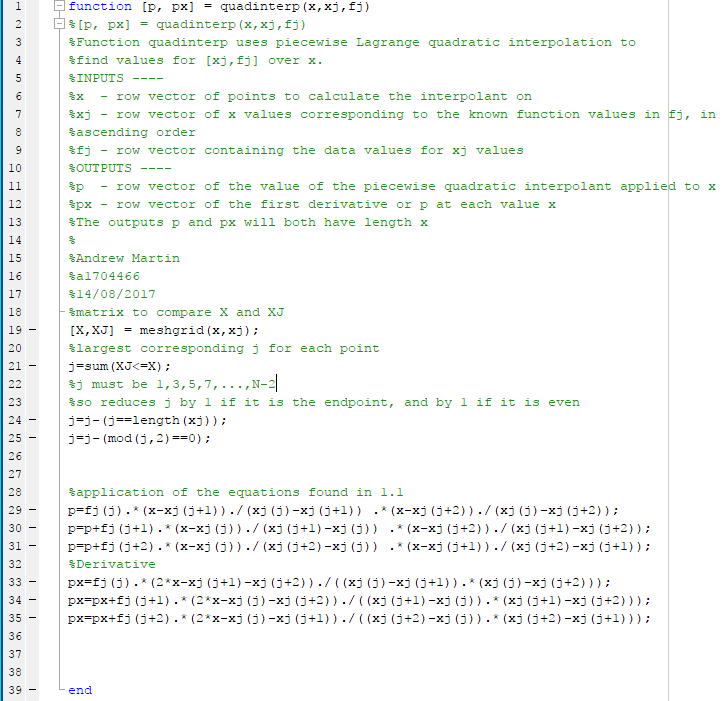
\includegraphics{quadinterp.PNG}
	
	
	
	
	\newpage
	Question 3\\
	Given equally-spaced data points find $N_{min}$ to approximate $f(x)=\cos^2(x)$ over $0\leq x\leq 2\pi$ to an accuracy of $10^{-1}$.
	
	Polynomial interpolation error has form:
	$$\epsilon_n(x) = f(x)-p_n(x) = \frac{f^{(n+1)}(t_x)}{(n+1)!}\prod_{j=0}^{n}(x-x_j)$$
	with $n$ points..
	We want 
	$$\epsilon \leq 10^{-1}$$
	$$\implies \max\left(\frac{f^{(n+1)}(t_x)}{(n+1)!}\prod_{j=0}^{n}(x-x_j)\right)\leq 10^{-1}$$
	Since we are using quadratic interpolation, this gives:
	$$=\max\left(\frac{4\sin(2t_x)}{3!}(x-x_0)(x-x_1)(x-x_2)\right)\leq 10^{-1}$$
	$$=\max\left(\frac{4\sin(2t_x)}{6}(x-x_0)(x-x_1)(x-x_2)\right)\leq 10^{-1}$$
	This can be transformed by letting $x-x_1 = y$ i.e. $x=y+x_1 $ and since $\pi/2 $ is contained in the interval, sin can be maximised to 1.
	$$\implies =\max\left(\frac{4}{6}(y+x_1-x_0)(y)(y+x_1-x_2)\right)\leq 10^{-1}$$
	Since the points are equally spaced, let $h=x_{j+1}-x_j$
	$$\implies =\max\left(\frac{2}{3}(y+h)(y)(y-h)\right)\leq 10^{-1}$$
	$$ =\max\left(\frac{2}{3}(y^3 - yh^2)\right)\leq 10^{-1}$$
	$$ \max {y^3 - yh^2} \implies 3y^2 -h^2 = 0 \implies y= \frac{h}{\sqrt{3}}$$
	$$ =\max\left(\frac{2}{3}((\frac{h}{3\sqrt{3}})^3 - \frac{h}{\sqrt{3}} h^2)\right)\leq 10^{-1}$$
	$$ =\max\left(\frac{2h^3}{9\sqrt{3}} - \frac{2h^3}{3\sqrt{3}} \right)\leq 10^{-1}$$
	We want the maximum value so we can take the absolute value of $-4h^3$
	$$ =\max\left(\frac{|-4h^3|}{9\sqrt{3}}\right)\leq 10^{-1}$$
$$ =\max\left(\frac{4h^3}{9\sqrt{3}}\right)\leq 10^{-1}$$
$N=1 + \frac{2\pi}{h} \implies h = \frac{2\pi}{N-1}$
$$ =\left(\frac{2\pi}{N-1}\right)^3 \left(\frac{4}{9\sqrt{3}}\right)\leq 10^{-1}$$
$$ \frac{2\pi}{N-1} \leq \sqrt[3]{\frac{9\sqrt{3}}{4}10^{-1}} $$
$$ 2\pi \leq \sqrt[3]{\frac{9\sqrt{3}}{4}10^{-1}} (N-1) $$
$$ \frac{2\pi}{\sqrt[3]{\frac{9\sqrt{3}}{4}10^{-1}}} \leq  (N-1) $$
$$N\geq \frac{2\pi}{\sqrt[3]{\frac{9\sqrt{3}}{4}10^{-1}}} +1 $$
	N min when this is equality (or as close to as possible).
	$N_{min} =  9.60 ...$ But $N_{min}$ must be an integer so the minimum value, and it must be odd since we are using interpolation so:
	$$N_{min} = 11$$
	
	
	
	
	
	
	\newpage
	Question 4\\
	MATLAB script quadtest to sample $f(x)=\cos^2(x)$ over $0\leq x\leq 2\pi$ then calls quadinterp from 1.2 to evaluate the interpolant and its first derivative on $1000$ equi-spaced points over the same interval.\\
	Create two plots\\
	
	(a) The absolute error i.e. $|f(x)-P(x)|$ over the domain (check the absolute error is bounded above by $10^{-1}$).\\
	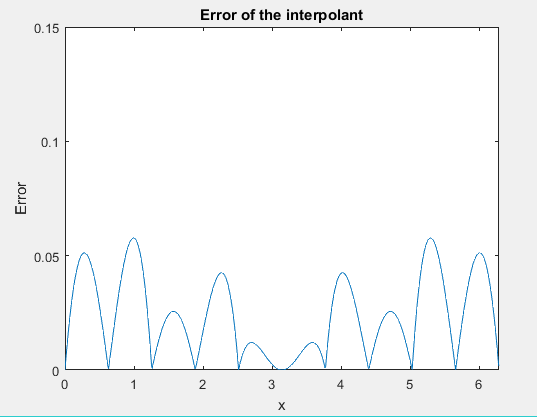
\includegraphics{errorgraph.PNG}\\
	Over the domain $0\leq x \leq 2\pi$, this is always under $0.1$.\\
	\newpage
	(b) The first derivatives $f'(x)$, $P'(x)$ over the interval\\
	
	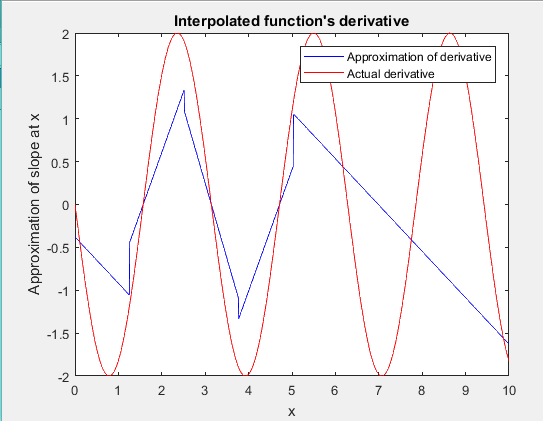
\includegraphics{plotderivatives.PNG}\\
	From this it is quite visible that there is significant error in the interpolated derivative.
	
	\newpage
	Question 5\\
	Using more points $N > N_{min}$, discuss the accuracy of the interpolant and derivative as N increases. 
	Explain why the derivative $P'(x)$ generically doesn't match $f'(x)$ as well as $P(x)$ matches $f(x)$\\
	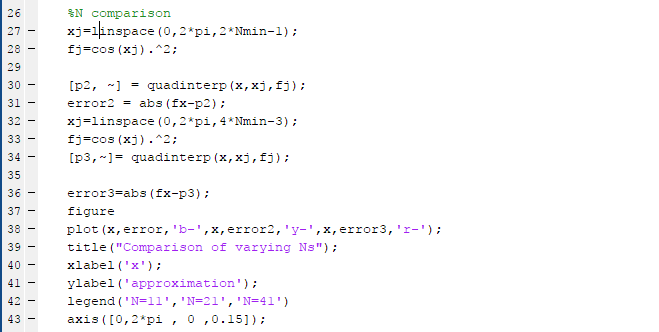
\includegraphics{Ncompare.png}
	From the maths done in question 3, and from the plot above, it is apparent that As N increases, the error of the approximation decreases.
	Doubling N (and subtracting $1$ to keep it odd), approximately decreases the error by a factor of 8. 
	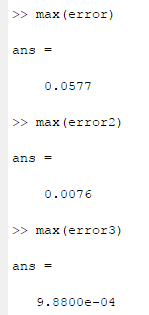
\includegraphics{errorcompare.png}
	\\
	
	The derivative $P'(x)$ won't usually match $f'(x)$. This is due to points where the derivative isn't defined - $P'(x)$ will have 2 values at the same point. I.e. for $x_j$, $j=1,3,5...$ the $j$ values $3,5,7,9...$ will have 2 values for the derivative. which means these points will have an undefined slope.
	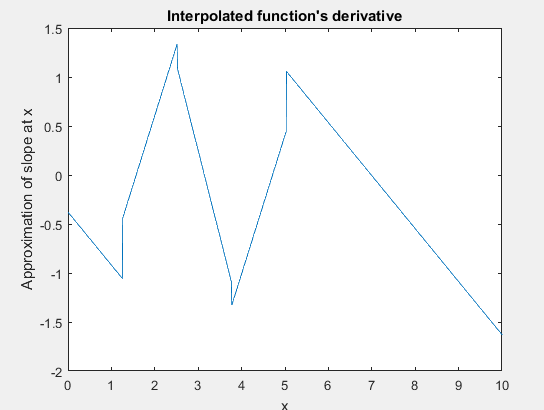
\includegraphics{plotderivative.PNG}
	As shown in the figure, close to the values $x=1,2.5,3.5,5$ the derivative has two values, which is apparent by the vertical lines.\\
	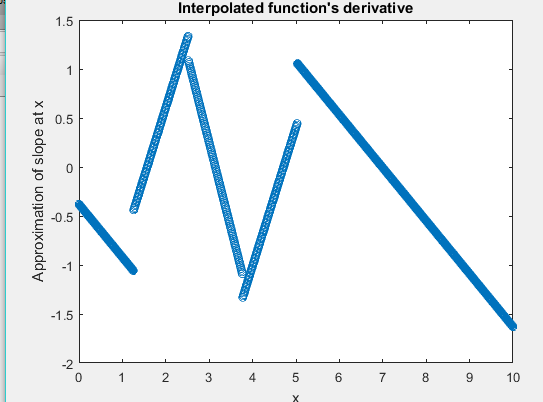
\includegraphics{plotderivativeclear.PNG}\\
	This image makes it clearer, as gaps are evident in the plot.
	
		\newpage
	Question 6\\
	Add more code to quadtest which loads bay\_city.dat and then calls quadinterp to interpolate the data and plot the elevation every $h=1m$ along the course. Plot the original points as circles or crosses and label axes meaningfully.
	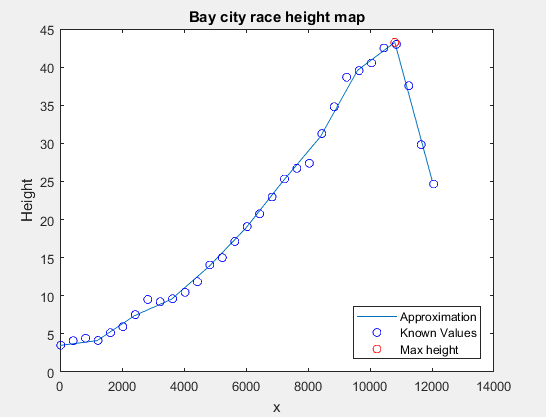
\includegraphics{baycityheight.PNG}
	\\
	Plot of an approximation of the height map of the bay-city run.
	
	\newpage
	Question 7\\
	add code which uses logical indexing to answer:\\
	(a) How far into the course is the highest elevation (function)
	\\
	As shown in the graphic in question 6, indicated with a red circle, the maximum height of the bay-city race is approximately $10800$m in or $10.8$Km, with an approximate height of  $43$m.\\

	(b) How far in is the steepest uphill part (derivative)\\
	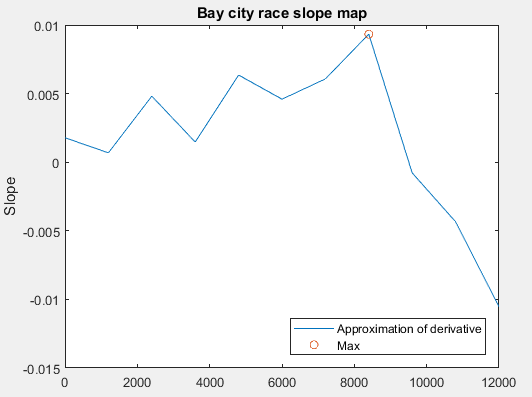
\includegraphics{baycityderiv.PNG}
	\\
	It was found (and is shown in the graph above) that the point with the maximum slope is $x=8400$m into the bay-city run. The slope at this point is $0.0093$m.
	
	
	\newpage
	Question 8\\
	Comment on a potential numerical issue with quadratic interpolation as defined in quadinterp in finding the steepest section of the course.\\
	As discussed in question 5 the derivative is not defined on the points $j=3,5,7,9,11$ 
	
	Another issue is there is no reference to compare the slope generated this way to the actual slope of the race. There is no given slope.
	
	\newpage
	Complete quadtest code:\\
	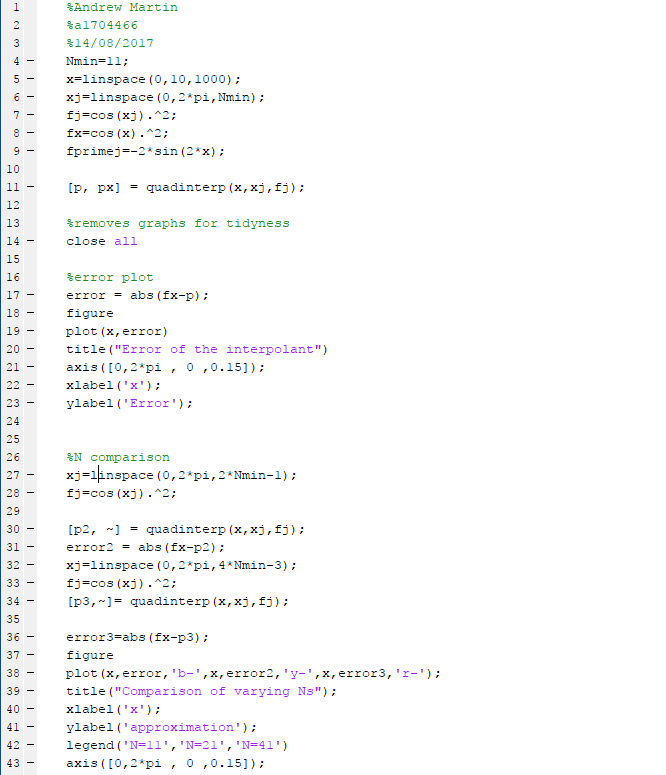
\includegraphics{quadtest1.PNG}
	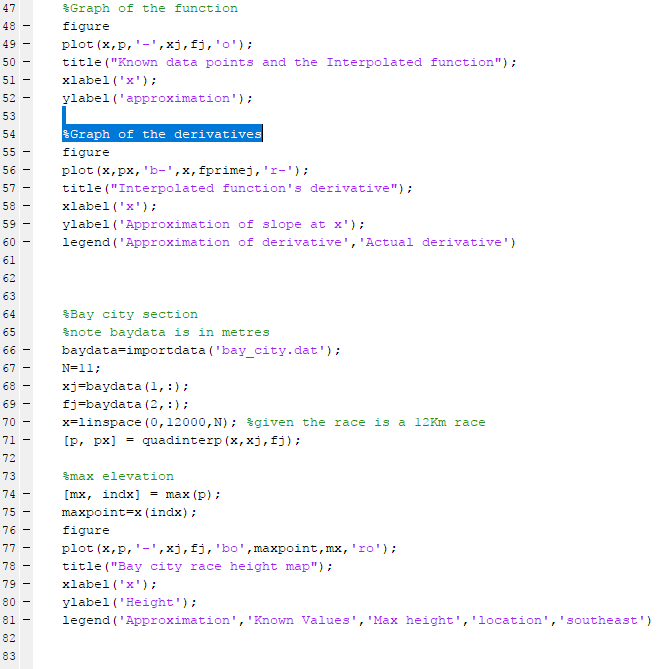
\includegraphics{quadtest2.PNG}
	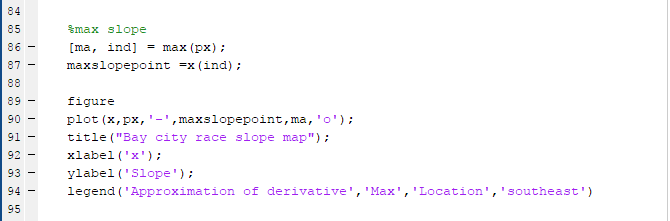
\includegraphics{quadtest3.PNG}

	
	
\end{document}